\begin{center}
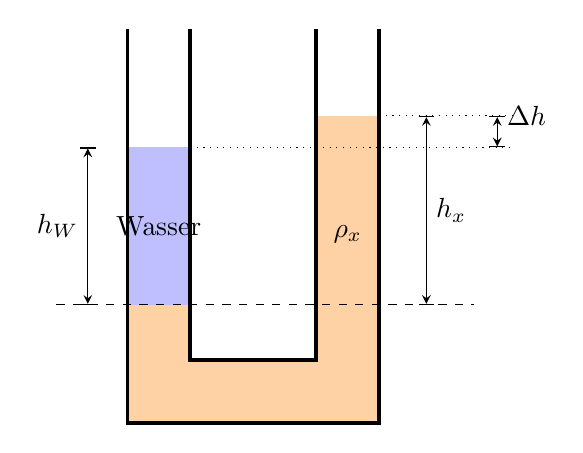
\begin{tikzpicture}[>=stealth]
 \fill[orange!35] (0,0) -- (0,1.5) -- (0.8,1.5) -- (0.8,0.8) -- (2.4,0.8) -- (2.4,3.9) -- (3.2,3.9) -- (3.2,0) -- cycle;
 \fill[blue!25] (0,1.5) rectangle (0.8,3.5);
 \draw[very thick] (0,5) -- (0,0) -- (3.2,0) -- (3.2,5);
 \draw[very thick] (0.8,5) -- (0.8,0.8) -- (2.4,0.8) -- (2.4,5);
 \node at (0.4,2.5) {Wasser};
 \node at (2.8,2.4) {$\rho_x$};
 \draw[dashed] (-0.9,1.5) -- (4.4,1.5);
 \draw[dotted] (0.8,3.5) -- (4.9,3.5);
 \draw[dotted] (3.2,3.9) -- (4.9,3.9);
 \draw[|<->|] (-0.5,1.5) -- (-0.5,3.5) node[midway, left] {$h_\text{W}$};
 \draw[|<->|] (3.8,1.5) -- (3.8,3.9) node[midway, right] {$h_x$};
 \draw[|<->|] (4.7,3.5) -- (4.7,3.9) node[right] {$\Delta h$};
\end{tikzpicture}
\end{center}
(nicht massstäblich)

Auf der Höhe der Trennfläche zwischen Wasser und unbekannter Flüssigkeit (gestrichelt) herrscht in beiden Schenkeln derselbe Druck. Über dieser Höhe steht links die Wassersäule $h_\text{W} = \hWO$, rechts eine Säule der unbekannten Flüssigkeit mit der Höhe $h_x = h_\text{W} + \Delta h$, da ihr Spiegel um $\Delta h = \hdiO$ höher liegt. Gleiche Schweredrücke bedeuten
\begin{align}
 \rho_\text{W}\,g\,h_\text{W} &= \rho_x\,g\left(h_\text{W}+\Delta h\right)
\end{align}
und mit $\rho_\text{W} = \rhoWO$ (FoTaBe S.~187)
\begin{align}
 \rho_x &= \rhoXF \\
   &= \frac{\hW}{\hW+\hdi}\cdot\rhoW \\
   &= \rhoX \approx \result{\rhoXP{0}{2}}
\end{align}
Das passt zu \result{\text{Olivenöl}} ($\rho = \rhoOlO$, FoTaBe S.~187).
